\documentclass[10pt,a4paper,twocolumn]{extarticle}
\usepackage[T1]{fontenc}
\usepackage[utf8]{inputenc}
\usepackage{lmodern}
\usepackage[a4paper,top=1.7cm,bottom=1.8cm,left=1.7cm,right=1.7cm,columnsep=0.6cm]{geometry}
\usepackage{microtype}
\usepackage{amsmath,amssymb}
\usepackage{booktabs,array}
\usepackage[table]{xcolor}
\usepackage{graphicx}
\usepackage{enumitem}
\usepackage{balance}
\usepackage{tikz}
\usetikzlibrary{arrows.meta,positioning,fit,backgrounds}
\definecolor{accent}{HTML}{184F95}
\usepackage[font=footnotesize,labelfont=bf,labelsep=period,justification=justified,singlelinecheck=false,skip=3pt]{caption}
\usepackage[colorlinks=true,linkcolor=accent,citecolor=accent,urlcolor=accent]{hyperref}
\usepackage{titlesec}
\titleformat{\section}{\normalsize\bfseries\color{accent}}{\thesection.}{0.5em}{}
\titleformat{\subsection}{\small\bfseries}{\thesubsection}{0.5em}{}
\titlespacing*{\section}{0pt}{7pt}{3pt}
\titlespacing*{\subsection}{0pt}{4pt}{2pt}
\setlist{itemsep=0pt,topsep=2pt,leftmargin=1.2em,parsep=0pt}
\setlength{\parskip}{0pt}
\setlength{\parindent}{1em}
\renewcommand{\arraystretch}{1.08}
\setlength{\textfloatsep}{8pt plus 2pt minus 2pt}
\setlength{\floatsep}{6pt plus 2pt minus 2pt}
\setlength{\intextsep}{6pt plus 2pt minus 2pt}
\setlength{\dbltextfloatsep}{8pt plus 2pt minus 2pt}
\setlength{\dblfloatsep}{6pt plus 2pt minus 2pt}
\newcolumntype{P}[1]{>{\raggedright\arraybackslash}p{#1}}
\newcommand{\good}[1]{\cellcolor{green!14}#1}
\newcommand{\fair}[1]{\cellcolor{yellow!22}#1}
\newcommand{\poor}[1]{\cellcolor{red!13}#1}
\newcommand{\nt}[1]{\cellcolor{black!06}#1}
\renewcommand{\thefigure}{\arabic{figure}}
\pagestyle{plain}

\begin{document}

\twocolumn[{%
\begin{center}
{\Large\bfseries UWB Anchor Self-Localization in 3D:\\[2pt]
Algorithm Comparison under Noise, Link Loss and NLOS}\\[8pt]
{\normalsize Bc. Inessa Davtyan}\\[2pt]
{\small Faculty of Electrical Engineering, Czech Technical University in Prague}\\[2pt]
{\small October 2026}
\end{center}
\vspace{-2pt}
\begin{center}
\begin{minipage}{0.92\textwidth}
\small\textbf{Abstract}\,---\,%
Ultra-wideband (UWB) positioning needs known anchor coordinates, but only the pairwise two-way ranges between anchors are
measured. This research compares four families of range-only 3D self-localization algorithms in Monte Carlo
simulation against the Cram\'er--Rao bound (CRB). Nonlinear least squares (NLS) initialized by classical MDS reaches the
CRB on clean data. Under link loss, a multi-start variant cuts gross failures from
30\,\% to 3\,\% at 20\,\% missing links. A soft-$\ell_1$ loss lowers the median error by 27--33\,\% at 5--10\,\% NLOS links.
Anchor sets with $\le2$\,m height spread have a vertical error 5 -- 6 times the horizontal one. The covariance $\sigma^2(\mathbf{J}^\top\mathbf{J})^+$
is calibrated: its 95\,\% ellipse covers 94\,\% of 400 Monte Carlo estimates.

\end{minipage}
\end{center}
\vspace{4pt}
}]

%% ---------------------------------------------------------------- I
\section{Introduction}
Surveying anchors by hand is slow, error-prone and must be repeated whenever the constellation changes~\cite{corbalan2023}.
Self-localization estimates anchor coordinates from the $N(N{-}1)/2$ inter-anchor ranges alone. The result is a
relative map: ranges fix the shape up to a rigid motion and a reflection (Fig.~\ref{fig:schema}b), so an absolute frame
needs additional reference points. This research asks which algorithm is accurate, robust to missing and biased links, cheap and
able to report its own uncertainty. Contributions:
\begin{itemize}
\item a literature overview and a unified formulation with an analytical bound,
\item a paired Monte Carlo comparison of six variants over noise, anchor count, link loss, NLOS and height (Figs.~\ref{fig:example}--\ref{fig:height}),
\item a calibrated covariance and a recommended pipeline (Fig.~\ref{fig:pipe}, Table~\ref{tab:matrix}).
\end{itemize}

%% ---------------------------------------------------------------- II
\section{Problem and Background}
\subsection{Model, objective, bound}
For anchors $x_1,\dots,x_N\in\mathbb{R}^3$ and a measured link set $\mathcal{E}$,
\begin{align}
d_{ij} &= \lVert x_i-x_j\rVert + n_{ij} + b_{ij},\quad n_{ij}\sim\mathcal{N}(0,\sigma^2),\; b_{ij}\ge 0, \label{eq:model}\\
\hat X &= \arg\min_X \sum_{(i,j)\in\mathcal{E}} \rho\!\left(\lVert x_i-x_j\rVert - d_{ij}\right), \label{eq:obj}
\end{align}
with $\rho(r)=r^2$ (least squares) or the soft-$\ell_1$ loss $\rho(r)=2f^2(\sqrt{1+(r/f)^2}-1)$, $f=0.3$\,m. With
$u_{ij}=(x_i-x_j)/\lVert x_i-x_j\rVert$ the Fisher information is
\begin{align}
\mathbf{J}_F&=\sigma^{-2}\!\!\sum_{(i,j)\in\mathcal{E}}\!(e_i-e_j)(e_i-e_j)^{\top}\!\otimes u_{ij}u_{ij}^{\top},\nonumber\\
\mathrm{RMSE}&\ge\sqrt{\mathrm{tr}(\mathbf{J}_F^{+})/N}. \label{eq:crb}
\end{align}
The pseudo-inverse removes the six rigid-motion modes. Unique realizability needs a (globally) rigid graph with $\ge 3N{-}6$ links and at
least four per node~\cite{aspnes2006,hendrickson1992}. Otherwise noise selects among flip solutions~\cite{moore2004}.



% \subsection{Related work}
% \textbf{Closed-form MDS} embeds the squared-distance matrix by eigendecomposition~\cite{torgerson1952}; shortest paths fill missing
% entries~\cite{shang2003}, and UWB systems use it directly~\cite{pourjabar2023,corbalan2023}. \textbf{Stress majorization}
% (SMACOF)~\cite{deleeuw2009,mair2022} handles missing entries but ends in local minima. \textbf{Least-squares refinement} over all ranges is common
% in UWB practice~\cite{queralta2020,almansa2020} and can include antenna delays~\cite{piavanini2022}; noise-induced flips are analysed in~\cite{moore2004}.
% \textbf{Semidefinite relaxations}~\cite{biswas2006,carter2006} need no initial guess but are much heavier. \textbf{Grid and particle filters} report
% sub-metre accuracy~\cite{schwarzbach2025} and below 15\,cm~\cite{koch2025} at higher cost. \textbf{Sensor-assisted} methods need a moving platform:
% UWB with IMU~\cite{shi2019}, SLAM~\cite{nguyen2025}, simulation~\cite{pereira2021}. Localizability and bounds follow from rigidity theory and Fisher
% information~\cite{aspnes2006,hendrickson1992,heng2013,jourdan2008}.

%% ---------------------------------------------------------------- III
\section{Methods}

\textbf{cMDS}: fill missing ranges by shortest paths, double-center the squared matrix, take the three largest eigenpairs.\\
\textbf{SMACOF}: weighted stress majorization from the cMDS start. \\\textbf{NLS/LM}: trust-region Levenberg--Marquardt on~\eqref{eq:obj} with
the analytic Jacobian, from the cMDS start. \textbf{Multi-start} adds seven random starts and keeps the lowest cost. \textbf{Soft-$\ell_1$} adds the robust loss.\\
\textbf{SDP}: anchor-free Gram-matrix relaxation (CVXPY/Clarabel), rank-3 projection, trace weight not tuned. Treated as an offline reference.\\


\par\vspace{3pt}\noindent\begin{minipage}{\columnwidth}
\centering
\captionof{table}{Compared estimators.}
\label{tab:algos}
\footnotesize
\setlength{\tabcolsep}{3pt}
\begin{tabular}{@{}P{1.9cm}P{2.1cm}P{1.8cm}P{1.35cm}@{}}
\toprule
Estimator & Principle & Missing links & Cost\\
\midrule
cMDS & closed form, $N^3$ & shortest paths & 1 EVD\\
SMACOF & majorization & weights & iterative\\
NLS/LM & Gauss--Newton family & only measured links & iterative\\
Multi-start (+ soft-$\ell_1$) & 8 NLS runs, min.\ cost & only measured links & $8\times$ NLS\\
SDP & convex relaxation & only measured links & interior point\\
\bottomrule
\end{tabular}
\end{minipage}\par\vspace{3pt}
\subsection{Experimental protocol}

\par\vspace{3pt}\noindent\begin{minipage}{\columnwidth}
\centering
\captionof{table}{Simulation settings.}
\label{tab:setup}
\footnotesize
\setlength{\tabcolsep}{3pt}
\begin{tabular}{@{}lP{6.0cm}@{}}
\toprule
Volume & uniform in $20\times20\times6$\,m, min.\ spacing 1\,m\\
Noise / defaults & $\sigma=10$\,cm, $N=8$, full mesh\\
Link loss & random removal, resampled until all nodes have $\ge4$ links and the framework is infinitesimally rigid\\
NLOS & fraction of links with bias $b\sim\mathcal{U}(0.5,2)$\,m\\
Trials & 60 per sweep point (40 in heatmaps), paired: all methods share data\\
Metric & RMSE after Procrustes alignment, gross failure = RMSE $>1$\,m\\
\bottomrule
\end{tabular}
\end{minipage}\par\vspace{3pt}

Table~\ref{tab:setup} lists the settings. Runtimes are desktop CPU, Python, and indicative only.

\twocolumn[{%
\begin{minipage}{\textwidth}
\centering
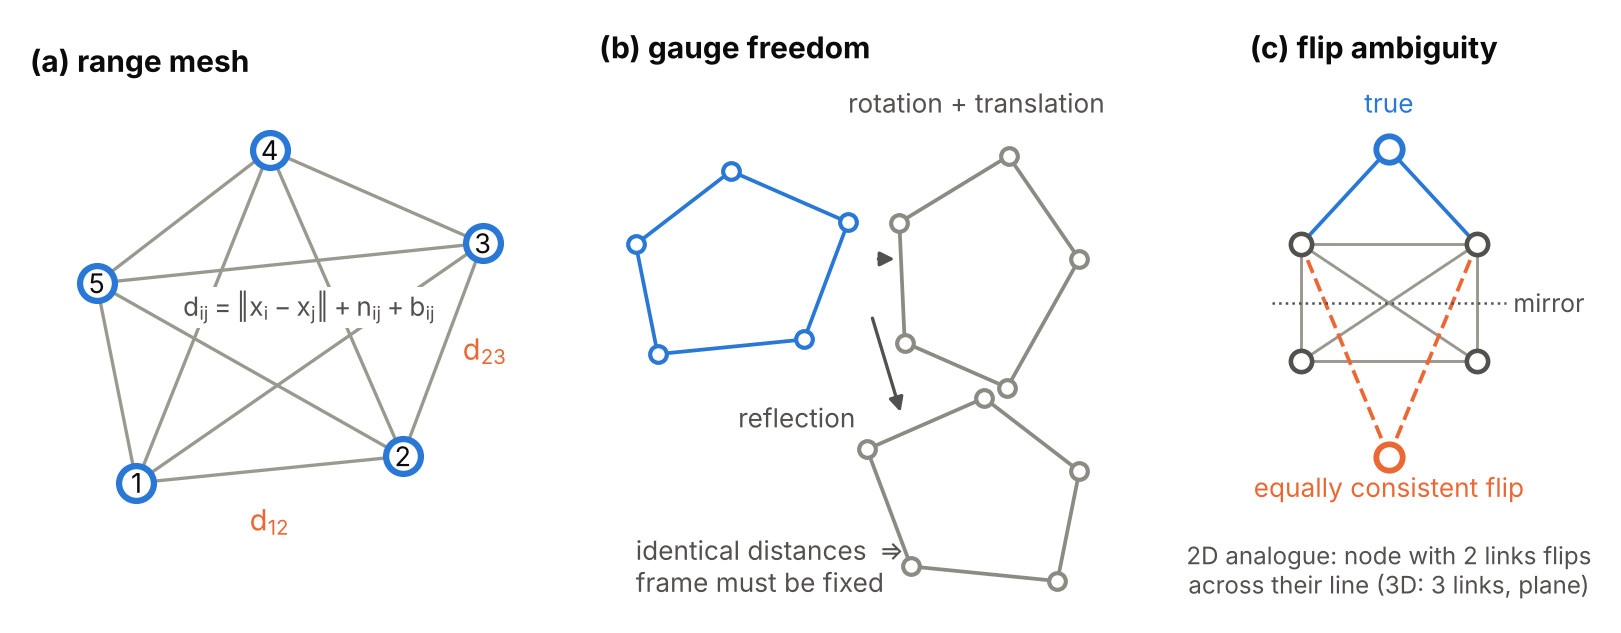
\includegraphics[width=\textwidth]{figures/f1_schematic.png}
\captionof{figure}{\textbf{Problem structure.} (a) Ranges $d_{ij}$ between all anchor pairs form the only input. (b) They are invariant under
rotation, translation and reflection, so a frame must be fixed externally. (c) Nodes with too few links can flip to a mirror
position that explains all ranges equally well.}
\label{fig:schema}
\end{minipage}
\par\vspace{3pt}
\begin{minipage}{\textwidth}
\centering
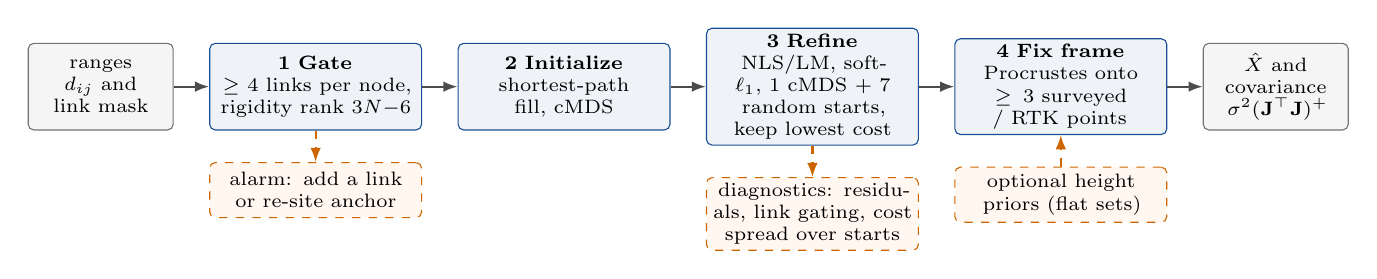
\begin{tikzpicture}[
  node distance=4.5mm,
  blk/.style={draw=accent,fill=accent!7,rounded corners=2pt,minimum height=11mm,text width=2.55cm,align=center,font=\scriptsize,inner sep=2pt},
  io/.style={draw=black!55,fill=black!4,rounded corners=2pt,minimum height=11mm,text width=1.7cm,align=center,font=\scriptsize,inner sep=2pt},
  opt/.style={draw=orange!80!black,dashed,fill=orange!6,rounded corners=2pt,minimum height=7mm,text width=2.55cm,align=center,font=\scriptsize,inner sep=2pt},
  arr/.style={-{Latex[length=1.8mm]},thick,black!70}]
\node[io] (in) {ranges $d_{ij}$ and link mask};
\node[blk,right=of in] (gate) {\textbf{1~Gate}\\ $\ge4$ links per node, rigidity rank $3N{-}6$};
\node[blk,right=of gate] (init) {\textbf{2~Initialize}\\ shortest-path fill, cMDS};
\node[blk,right=of init] (ref) {\textbf{3~Refine}\\ NLS/LM, soft-$\ell_1$, 1 cMDS + 7 random starts, keep lowest cost};
\node[blk,right=of ref] (frame) {\textbf{4~Fix frame}\\ Procrustes onto $\ge3$ surveyed / RTK points};
\node[io,right=of frame] (out) {$\hat X$ and covariance $\sigma^2(\mathbf{J}^\top\mathbf{J})^+$};
\foreach \a/\b in {in/gate,gate/init,init/ref,ref/frame,frame/out} \draw[arr] (\a)--(\b);
\node[opt,below=4mm of gate] (alarm) {alarm: add a link or re-site anchor};
\node[opt,below=4mm of ref] (diag) {diagnostics: residuals, link gating, cost spread over starts};
\node[opt,below=4mm of frame] (prior) {optional height priors (flat sets)};
\draw[arr,dashed,orange!80!black] (gate)--(alarm);
\draw[arr,dashed,orange!80!black] (ref)--(diag);
\draw[arr,dashed,orange!80!black] (prior)--(frame);
\end{tikzpicture}
\captionof{figure}{\textbf{Recommended pipeline.} Solid blocks are evaluated here. Dashed blocks are operational add-ons.}
\label{fig:pipe}
\end{minipage}
\par\vspace{3pt}
\begin{minipage}{\textwidth}
\centering
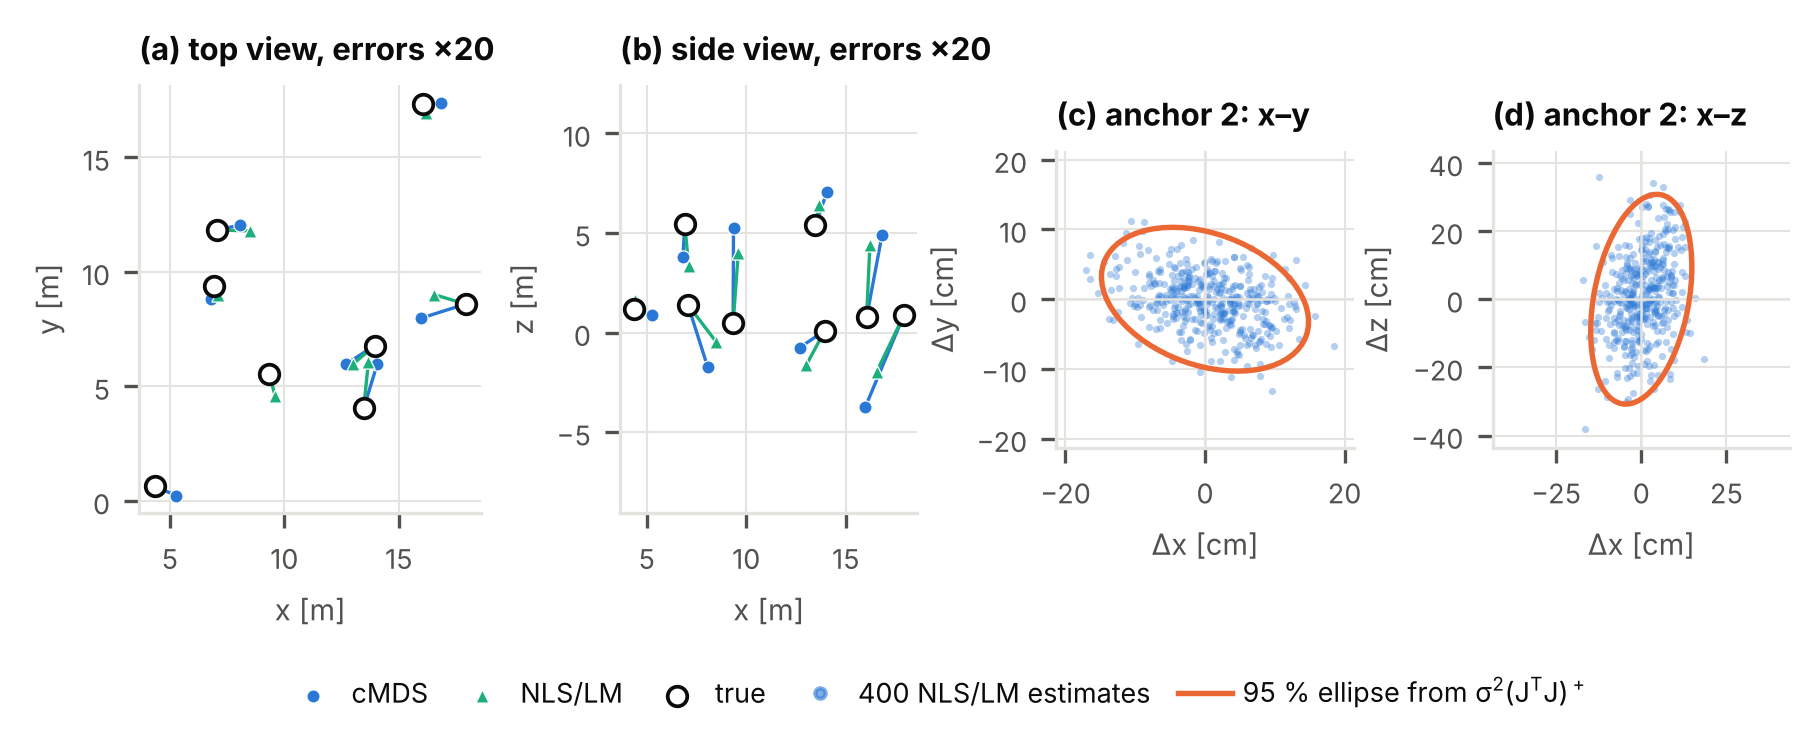
\includegraphics[width=\textwidth]{figures/f3_example_cov.png}
\captionof{figure}{\textbf{One constellation, many trials.} (a, b) Estimates of cMDS and NLS/LM for one noisy mesh ($N{=}8$), errors magnified $20\times$.
(c, d) 400 repeated noisy meshes of the same layout: scatter of the NLS/LM error of anchor~2 and the 95\,\% ellipse predicted by
$\sigma^2(\mathbf{J}^\top\mathbf{J})^+$. The ellipse contains 94\,\% of the estimates. The vertical spread (1$\sigma\approx$ 13\,cm) is twice the horizontal one (6\,cm).}
\label{fig:example}
\end{minipage}
\vspace{6pt}
}]
%% ---------------------------------------------------------------- IV
\section{Results}
\textbf{Key findings.}
\begin{enumerate}
\item NLS/LM reaches the CRB on clean data. cMDS is 17--30\,\% above it (Fig.~\ref{fig:noise}).
\item The CRB-based covariance is calibrated (94\,\% coverage, Fig.~\ref{fig:example}).
\item Multi-start removes gross failures up to 30\,\% link loss. The final cost identifies the flip (Figs.~\ref{fig:missing}--\ref{fig:heat},~\ref{fig:ecdf}).
\item Soft-$\ell_1$ helps at 5--10\,\% NLOS only (Fig.~\ref{fig:missing}c,d).
\item Vertical error dominates unless the anchors span $\ge4$\,m in height (Fig.~\ref{fig:height}).
\item Cost grows 12--16$\times$ from single to multi-start (Fig.~\ref{fig:pareto}).
\end{enumerate}

\par\vspace{3pt}\noindent\begin{minipage}{\columnwidth}
\centering
\captionof{table}{\textbf{Median RMSE vs.\ noise} ($N{=}8$, cm). NLS/LM stays within $\pm9$\,\% of the CRB. cMDS is 13--27\,\% above it.}
\label{tab:noise}
\footnotesize
\setlength{\tabcolsep}{4pt}
\begin{tabular}{@{}rrrrr@{}}
\toprule
$\sigma$ & CRB & NLS/LM & cMDS & SDP\\
\midrule
2 & 3.3 & 3.0 & 3.7 & 3.9\\
5 & 8.3 & 7.5 & 9.6 & 10.5\\
10 & 16.2 & 17.0 & 19.9 & 20.9\\
15 & 24.8 & 22.5 & 29.3 & 29.9\\
20 & 36.9 & 35.5 & 44.6 & 46.1\\
30 & 50.7 & 51.6 & 64.6 & 64.2\\
\bottomrule
\end{tabular}
\end{minipage}\par\vspace{3pt}

\twocolumn[{%
\begin{minipage}{\textwidth}
\centering
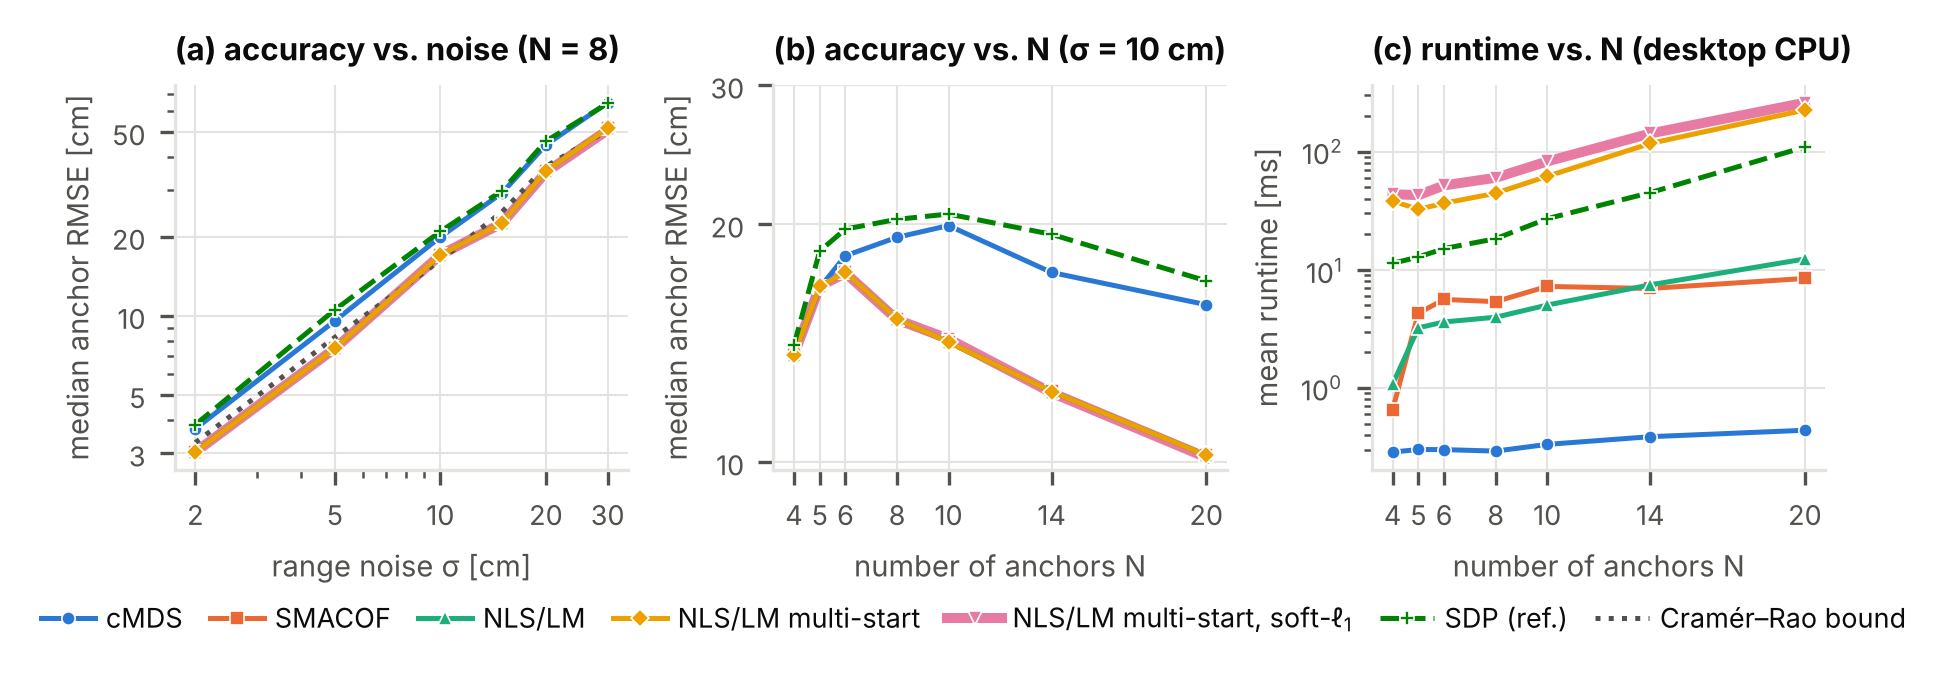
\includegraphics[width=\textwidth]{figures/f4_noise_nodes.png}
\captionof{figure}{\textbf{Clean-data accuracy and cost.} Median over 60 trials. NLS/LM and SMACOF follow the CRB. cMDS and SDP are
17--30\,\% above it. More anchors help NLS (14 cm at $N{=}10$ $\to$ 10 cm at $N{=}20$) but not cMDS. Cost: 0.3\,ms (cMDS), 1--12\,ms (NLS), 30--260\,ms (multi-start).}
\label{fig:noise}
\end{minipage}
\par\vspace{3pt}
\begin{minipage}{\textwidth}
\centering
\captionof{table}{\textbf{Summary.} Clean: $N{=}8$, $\sigma{=}10$\,cm. Stress: $N{=}12$, 20\,\% missing links and 10\,\% NLOS links. Failure = RMSE $>1$\,m.}
\label{tab:summary}
\footnotesize
\setlength{\tabcolsep}{5pt}
\begin{tabular}{@{}lrrrrrrr@{}}
\toprule
 & \multicolumn{2}{c}{clean} & \multicolumn{2}{c}{20\,\% links missing} & \multicolumn{2}{c}{10\,\% NLOS links} & runtime\\
\cmidrule(lr){2-3}\cmidrule(lr){4-5}\cmidrule(lr){6-7}
Method & median [cm] & p90 [cm] & median [cm] & failures [\%] & median [cm] & failures [\%] & $N{=}10$ [ms]\\
\midrule
cMDS & 19.9 & 31.4 & 302 & \poor{100} & 68 & \poor{25} & 0.3\\
SMACOF & 17.0 & 28.7 & 47 & \poor{33} & 63 & \poor{23} & 7.2\\
NLS/LM (cMDS init) & 17.0 & 28.7 & 23 & \poor{30} & 63 & \poor{23} & 5.0\\
NLS/LM multi-start & 17.0 & 28.7 & 20 & \good{3} & 63 & \fair{20} & 61.8\\
NLS/LM multi-start, soft-$\ell_1$ & 17.0 & 28.9 & 20 & \good{2} & 46 & \fair{17} & 82.6\\
SDP (reference) & 20.9 & 33.1 & 27 & \good{2} & 56 & \fair{20} & 27.1\\
\midrule
Cram\'er--Rao bound & 16.2 & & & & & &\\
\bottomrule
\end{tabular}
\end{minipage}
\par\vspace{3pt}
\begin{minipage}{\textwidth}
\centering
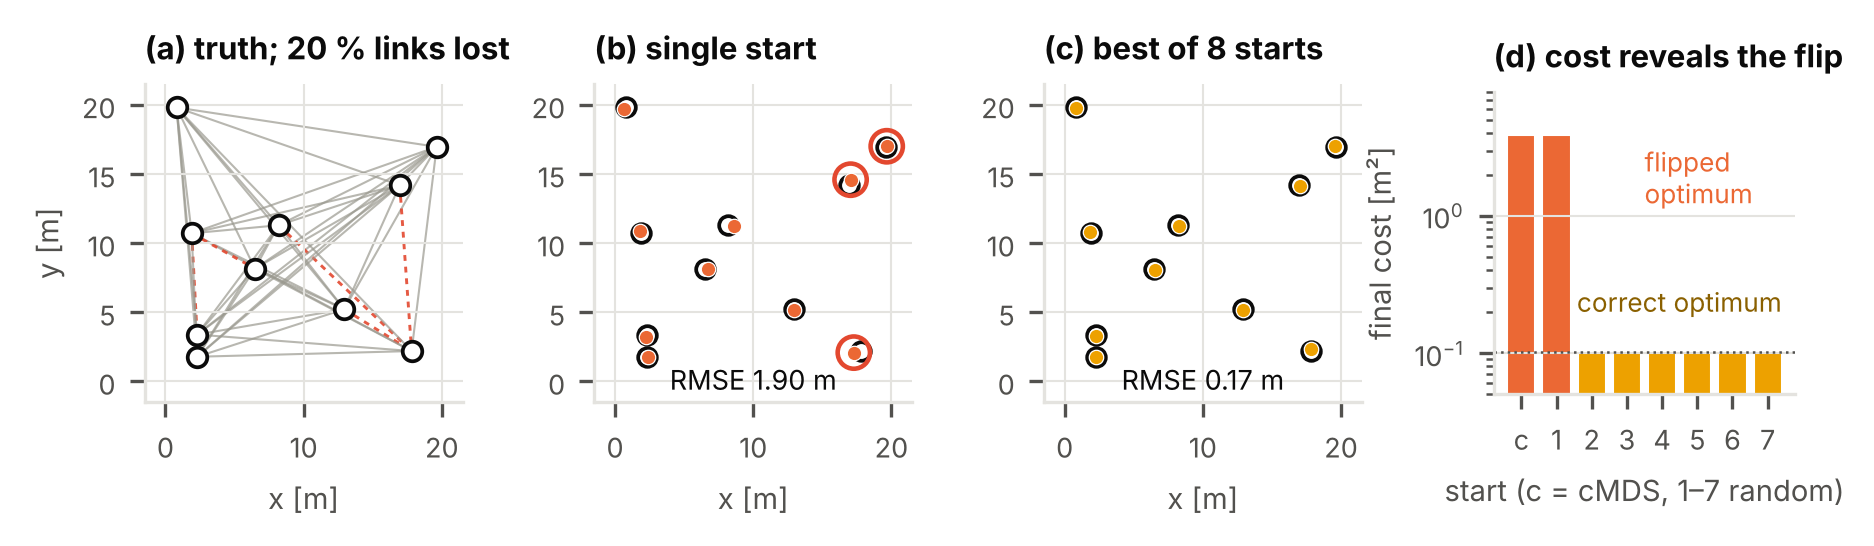
\includegraphics[width=\textwidth]{figures/f10_failure.png}
\captionof{figure}{\textbf{Anatomy of a gross failure} ($N{=}10$, 20\,\% links lost, one trial). (a) Truth and lost links (red dashed). (b) Single-start NLS/LM from the cMDS start
converges to a flipped configuration with three anchors off (red circles). (c) The best of eight starts is correct. (d) The final cost separates the two optima by a factor of 38,
so the lowest-cost start is a reliable selector here.}
\label{fig:fail}
\end{minipage}
}]

\par\vspace{3pt}\noindent\begin{minipage}{\columnwidth}
\centering
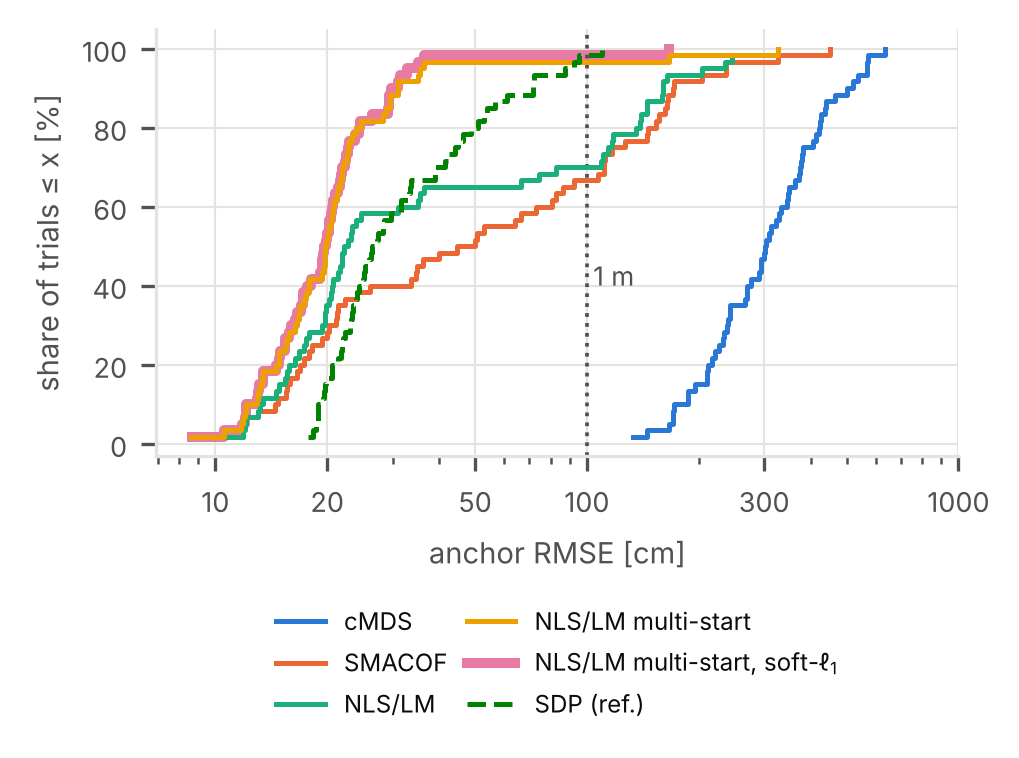
\includegraphics[width=\columnwidth]{figures/f8_ecdf.png}
\captionof{figure}{\textbf{Distribution of errors} at 20\,\% link loss ($N{=}12$). The multi-start curves rise steeply at 20\,cm. Single-start
methods have a heavy tail beyond 1\,m.}
\label{fig:ecdf}
\end{minipage}\par\vspace{3pt}

\par\vspace{3pt}\noindent\begin{minipage}{\columnwidth}
\centering
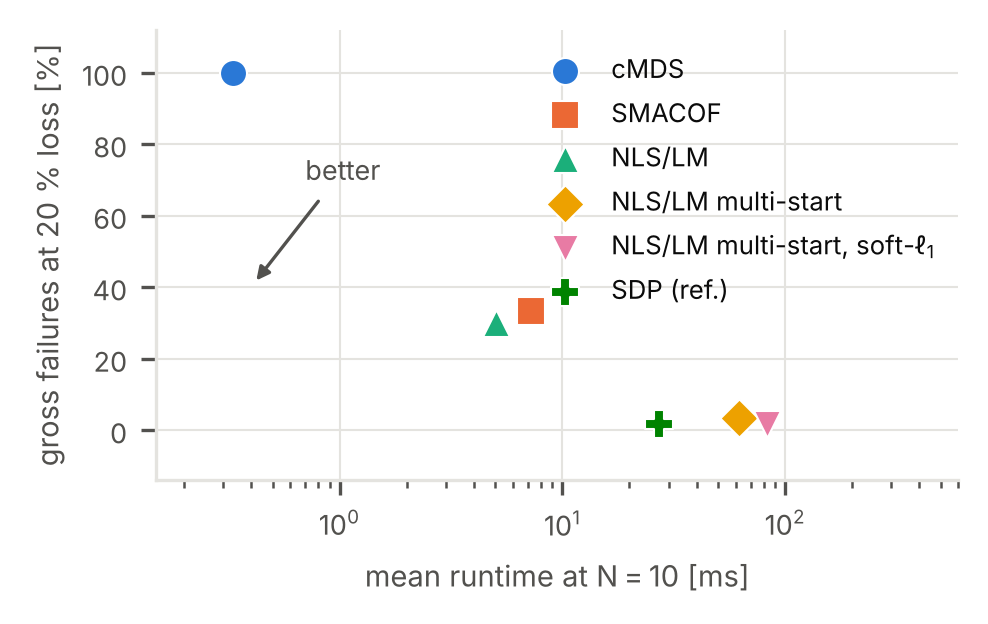
\includegraphics[width=\columnwidth]{figures/f9_pareto.png}
\captionof{figure}{\textbf{Robustness vs.\ cost.} Multi-start variants and SDP sit in the low-failure region. Multi-start NLS costs
$\sim$12--16$\times$ a single NLS run (desktop CPU, $N{=}10$).}
\label{fig:pareto}
\end{minipage}\par\vspace{3pt}

\twocolumn[{%
\begin{minipage}{\textwidth}
\centering
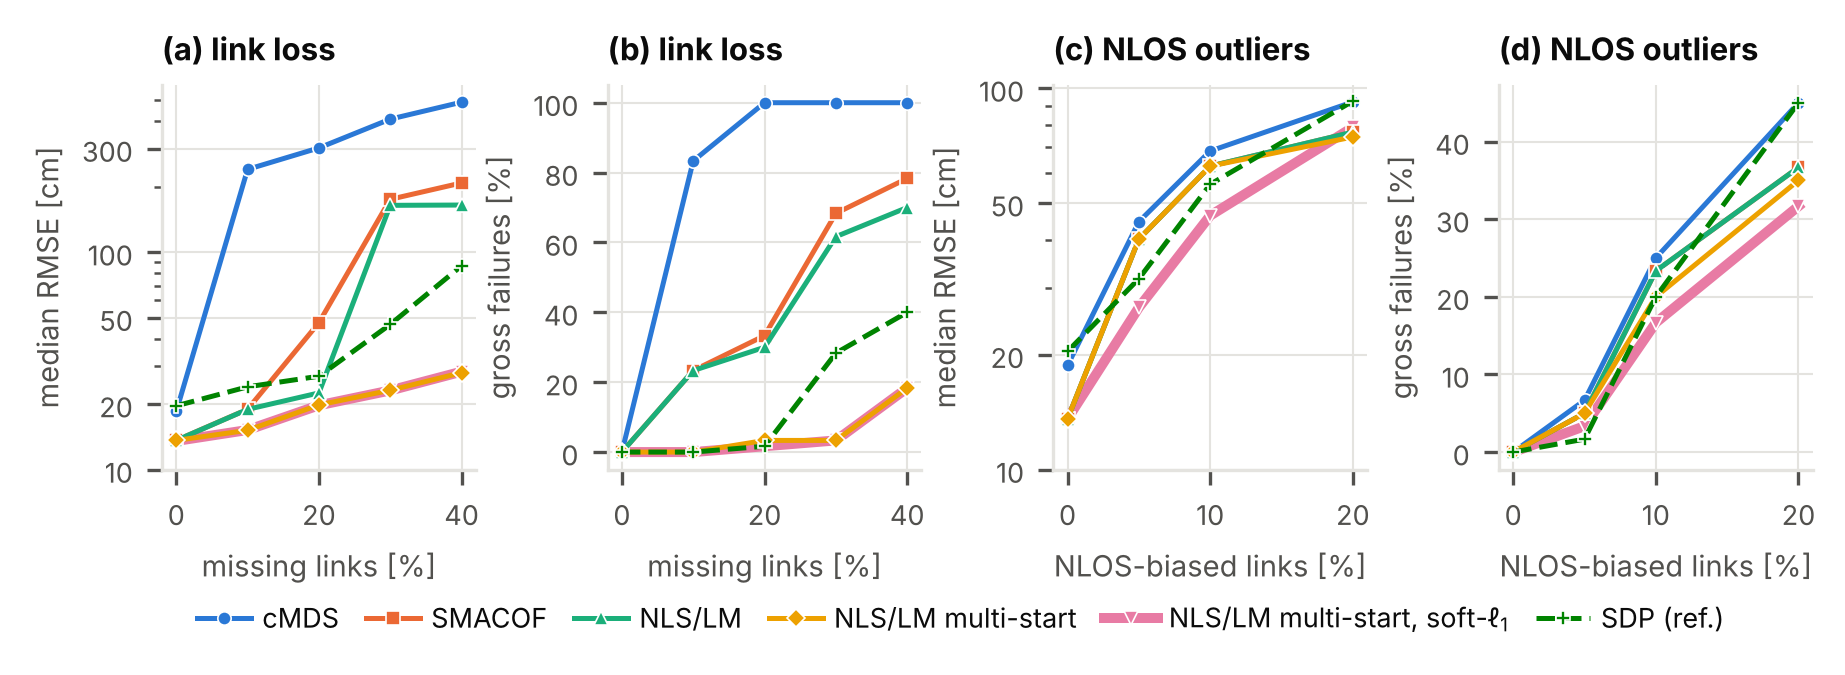
\includegraphics[width=\textwidth]{figures/f5_missing_nlos.png}
\captionof{figure}{\textbf{Missing links and NLOS} ($N{=}12$, 60 trials). cMDS fails from 10\,\% link loss on because shortest-path
fill inflates distances. Multi-start keeps failures $\le3$\,\% up to 30\,\% loss. The soft-$\ell_1$ loss helps at 5--10\,\% NLOS
(27 vs.\ 40\,cm at 5\,\%) and not at 20\,\%, where no method works.}
\label{fig:missing}
\end{minipage}
\par\vspace{3pt}
\begin{minipage}{\textwidth}
\centering
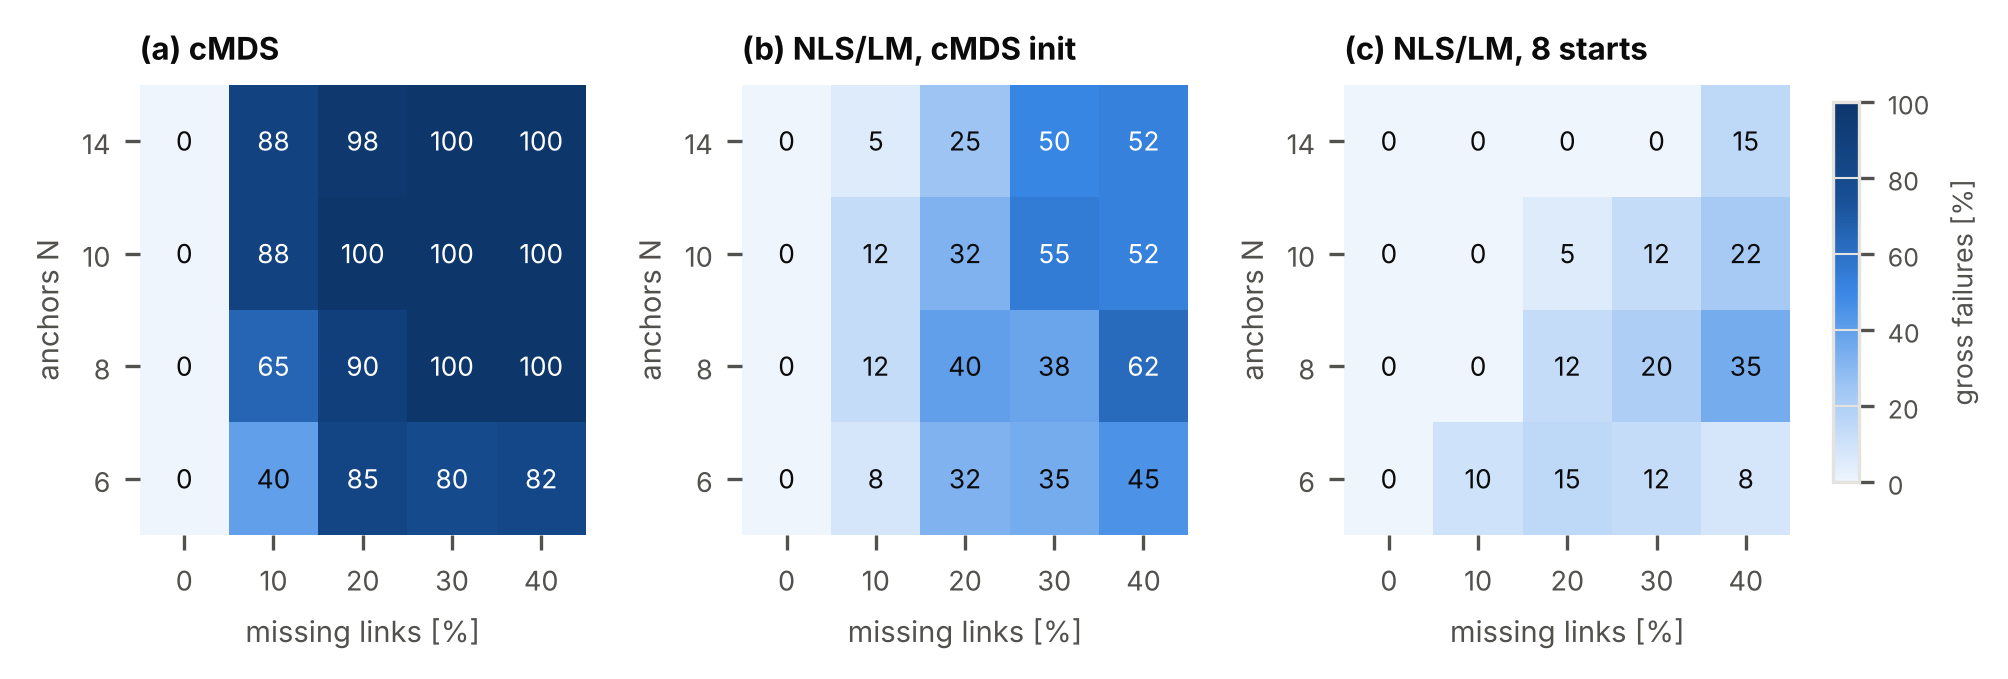
\includegraphics[width=\textwidth]{figures/f6_heatmaps.png}
\captionof{figure}{\textbf{Failure rate over anchor count and link loss} (40 trials per cell). Single-start refinement fails in 25--55\,\% of the
meshes at 20--30\,\% loss for every $N$. Eight starts remove most failures. Binomial s.e.\ is up to 8\,pp per cell.}
\label{fig:heat}
\end{minipage}
\par\vspace{3pt}
\begin{minipage}{\textwidth}
\centering
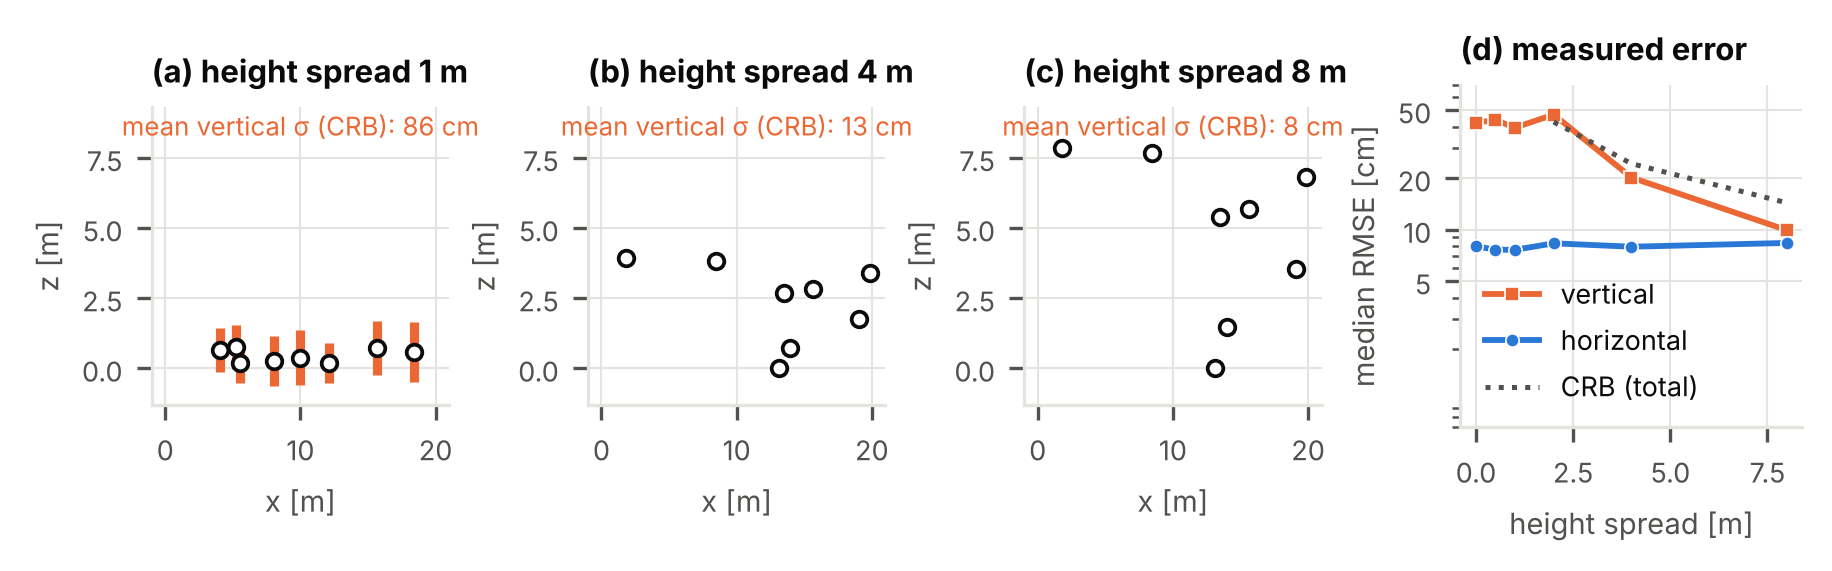
\includegraphics[width=\textwidth]{figures/f11_height_geometry.png}
\captionof{figure}{\textbf{Anchor height spread} ($N{=}8$). (a--c) Side views of three constellations. The bar length would be the CRB vertical standard deviation
(mean value printed). (d) Measured median error of the NLS multi-start soft-$\ell_1$ estimator: horizontal error stays at 8\,cm. Vertical error is 5--6$\times$ larger up to
2\,m height spread, 2.5$\times$ at 4\,m and 1.2$\times$ at 8\,m. The CRB (total) is shown only where it is well conditioned.}
\label{fig:height}
\end{minipage}
}]
\textbf{Link loss.} At 20\,\% loss the cMDS start is wrong in every trial, so single-start refinement inherits a
flipped or folded configuration in 30\,\% of the meshes (Fig.~\ref{fig:ecdf}). The lowest-cost start rescues almost all of them
(Fig.~\ref{fig:fail}d). Even eight starts fail in 8--15\,\% of the meshes at $N{=}6$ and in up to 35\,\% at 40\,\% loss (Fig.~\ref{fig:heat}).


\textbf{Cost.} Multi-start multiplies the runtime by the number of starts. Since random starts converge to the same optimum in
clean data, an early exit once two starts agree would recover most of the speed.


%% ---------------------------------------------------------------- V
\section{Discussion}

 NLS/LM over all ranges, cMDS-initialized, soft-$\ell_1$ loss, multi-start when the mesh is incomplete
(Fig.~\ref{fig:pipe}). It reaches the CRB, is the most robust option tested at moderate link loss, and gives a covariance for free.
Why not SDP? Comparable robustness to link loss but 23--40\,\% less accurate here (trace weight untuned), $\sim$5$\times$ slower than a single NLS.
Procrustes onto $\ge3$ surveyed points gives an absolute frame. Reference quality then adds directly to the error budget.


\twocolumn[{%
\begin{minipage}{\textwidth}
\centering
\captionof{table}{\textbf{Decision matrix.} Shading: green = good, yellow = acceptable, red = poor. Grey = literature only, not tested.}
\label{tab:matrix}
\footnotesize
\setlength{\tabcolsep}{4pt}
\begin{tabular}{@{}P{3.3cm}P{2.6cm}P{3.2cm}P{2.3cm}P{2.1cm}P{2.6cm}@{}}
\toprule
Method & Clean accuracy & Missing links & NLOS (10\,\%) & Compute & Covariance\\
\midrule
cMDS & \fair{17--30\,\% above NLS} & \poor{83\,\% fail at 10\,\% loss} & \poor{68\,cm} & \good{0.3\,ms} & \poor{none}\\
SMACOF & \good{at CRB} & \fair{33\,\% fail at 20\,\%} & \poor{63\,cm} & \good{7\,ms} & \poor{none}\\
NLS/LM, cMDS init & \good{at CRB} & \fair{30\,\% fail at 20\,\%} & \poor{63\,cm} & \good{5\,ms} & \good{$\sigma^2(\mathbf{J}^\top\mathbf{J})^+$}\\
NLS/LM multi-start, soft-$\ell_1$ & \good{at CRB} & \good{2\,\% fail at 20\,\%} & \fair{46\,cm} & \fair{83\,ms} & \good{$\sigma^2(\mathbf{J}^\top\mathbf{J})^+$}\\
SDP & \fair{23--40\,\% above NLS} & \good{2\,\% at 20\,\%, 28\,\% at 30\,\%} & \poor{56\,cm} & \fair{27\,ms} & \poor{none}\\
Grid / particle filter~\cite{schwarzbach2025,koch2025} & \nt{$<15$\,cm reported} & \nt{reported robust} & \nt{reported robust} & \nt{heavy} & \nt{posterior}\\
\bottomrule
\end{tabular}
\end{minipage}
}]
\textbf{Limitations.} Simulation only. Gaussian noise and uniform positive NLOS bias, no antenna-delay error.
Random volumes. Runtime not measured on embedded hardware. Multi-start cannot detect
a consistent flip, and soft-$\ell_1$ helps little above 10\,\% NLOS. Height priors and dynamic anchor counts were not simulated.



\par\vspace{3pt}\noindent\begin{minipage}{\columnwidth}
\centering
\captionof{table}{\textbf{Practical guidelines} derived from the experiments.}
\label{tab:rules}
\footnotesize
\setlength{\tabcolsep}{3pt}
\begin{tabular}{@{}P{1.35cm}P{3.0cm}P{3.9cm}@{}}
\toprule
Factor & Evidence & Guideline\\
\midrule
Links & single start fails 25--55\,\% at 20--30\,\% loss & $\ge4$ links per node, rigid, use multi-start below full mesh.\\
Height & vertical error 5--6$\times$ horizontal at $\le2$\,m & Spread anchors over $\ge4$\,m or add measured height priors.\\
NLOS & soft-$\ell_1$ gains 27--33\,\% at 5--10\,\% & Gate suspicious links, do not expect help above 10\,\%.\\
Count & 14\,cm ($N{=}10$) $\to$ 10\,cm ($N{=}20$) & More anchors reduce error, 8 is a workable minimum.\\
Frame & Procrustes needs $\ge3$ non-collinear points & Survey or RTK three anchors.\\
\bottomrule
\end{tabular}
\end{minipage}\par\vspace{3pt}
%% ---------------------------------------------------------------- VI
\section{Conclusion}
Range-only 3D anchor self-localization is best solved by robust, multi-start NLS refinement of an MDS initial guess. It matches the CRB,
survives 20--30\,\% link loss and cuts the damage of moderate NLOS by about 30\,\%, at tens of milliseconds on a desktop CPU. The dominant residual risks
are flat constellations (vertical error) and heavy NLOS contamination. Both call for geometry design and link gating rather than a different estimator.


{\footnotesize\setlength{\itemsep}{0pt}
\begin{thebibliography}{99}
\setlength{\itemsep}{0pt}\setlength{\parsep}{0pt}
\bibitem{nguyen2025} T.-D. Nguyen, T.-M. Nguyen, V.-H. Nguyen, ``Coordinate-consistent localization via continuous-time calibration and fusion of UWB and SLAM observations,'' arXiv:2510.05992, 2025. \url{https://arxiv.org/abs/2510.05992}

\bibitem{corbalan2023} P. Corbalan, G. P. Picco, M. Coors, V. Jain, ``Self-localization of ultra-wideband anchors: From theory to practice,'' \emph{IEEE Access}, vol.~11, pp.~29711--29725, 2023. doi:10.1109/ACCESS.2023.3261567

\bibitem{aspnes2006} J. Aspnes, T. Eren, D. K. Goldenberg, A. S. Morse, W. Whiteley, Y. R. Yang, B. D. O. Anderson, P. N. Belhumeur, ``A theory of network localization,'' \emph{IEEE Trans. Mobile Computing}, vol.~5, no.~12, Dec.\ 2006.

\bibitem{queralta2020} J. Pe\~na Queralta, C. Mart\'inez Almansa, F. Schiano, D. Floreano, T. Westerlund, ``UWB-based system for UAV localization in GNSS-denied environments: Characterization and dataset,'' 2020, arXiv:2003.04380; doi:10.1109/IROS45743.2020.9341042. \url{https://arxiv.org/abs/2003.04380}

\bibitem{pourjabar2023} M. Pourjabar, A. AlKatheeri, M. Rusci, A. Barcis, V. Niculescu, E. Ferrante, D. Palossi, L. Benini, ``Land \& Localize: An infrastructure-free and scalable nano-drones swarm with UWB-based localization,'' arXiv:2307.10255, 2023. \url{https://arxiv.org/abs/2307.10255}

\bibitem{hendrickson1992} B. Hendrickson, ``Conditions for unique graph realizations,'' \emph{SIAM J. Comput.}, vol.~21, no.~1, pp.~65--84, 1992.

\bibitem{moore2004} D. Moore, J. Leonard, D. Rus, S. Teller, ``Robust distributed network localization with noisy range measurements,'' in \emph{Proc. ACM SenSys}, 2004. \url{https://people.csail.mit.edu/teller/pubs/MooreEtAlSensys2004.pdf}

\bibitem{heng2013} L. Heng, G. X. Gao, ``Accuracy of range-based cooperative localization in wireless sensor networks: A lower bound analysis,'' arXiv:1305.7272, 2013. \url{https://arxiv.org/abs/1305.7272}

\bibitem{jourdan2008} D. B. Jourdan, D. Dardari, M. Z. Win, ``Position error bound for UWB localization in dense cluttered environments,'' \emph{IEEE Trans. Aerosp. Electron. Syst.}, 2008. \url{https://winslab.lids.mit.edu/wp-content/papercite-data/pdf/joudarwin-j08.pdf}

\bibitem{torgerson1952} W. S. Torgerson, ``Multidimensional scaling: I. Theory and method,'' \emph{Psychometrika}, vol.~17, no.~4, pp.~401--419, 1952.

\bibitem{shang2003} Y. Shang, W. Ruml, Y. Zhang, M. P. J. Fromherz, ``Localization from mere connectivity,'' in \emph{Proc. ACM MobiHoc}, pp.~201--212, 2003.

\bibitem{deleeuw2009} J. de Leeuw, P. Mair, ``Multidimensional scaling using majorization: SMACOF in R,'' \emph{J. Stat. Softw.}, vol.~31, no.~3, 2009. \url{https://www.jstatsoft.org/v31/i03}

\bibitem{mair2022} P. Mair, P. J. F. Groenen, J. de Leeuw, ``More on multidimensional scaling in R: smacof version 2,'' \emph{J. Stat. Softw.}, vol.~102, no.~10, pp.~1--47, 2022. doi:10.18637/jss.v102.i10

\bibitem{biswas2006} P. Biswas, T.-C. Liang, T.-C. Wang, Y. Ye, ``Semidefinite programming based algorithms for sensor network localization,'' \emph{ACM Trans. Sensor Networks}, 2006. doi:10.1145/1149283.1149286

\bibitem{carter2006} M. W. Carter, H. H. Jin, M. A. Saunders, Y. Ye, ``SpaseLoc: An adaptive subproblem algorithm for scalable wireless sensor network localization,'' \emph{SIAM J. Optim.}, vol.~17, no.~4, pp.~1102--1128, 2006. doi:10.1137/040621600

\bibitem{almansa2020} C. Mart\'inez Almansa, W. Shule, J. Pe\~na Queralta, T. Westerlund, ``Autocalibration of a mobile UWB localization system for ad-hoc multi-robot deployments in GNSS-denied environments,'' arXiv:2004.06762, 2020. \url{https://arxiv.org/abs/2004.06762}

\bibitem{piavanini2022} M. Piavanini, L. Barbieri, M. Brambilla, M. Cerutti, M. Nicoli, ``A calibration method for antenna delay estimation and anchor self-localization in UWB systems,'' 2022. \url{https://re.public.polimi.it/handle/11311/1221088}

\bibitem{schwarzbach2025} P. Schwarzbach, A. Jung, ``Evaluation of grid-based uncertainty propagation for collaborative self-calibration in indoor positioning systems,'' arXiv:2511.10526, 2025. \url{https://arxiv.org/abs/2511.10526}

\bibitem{koch2025} Koch, thesis on automatic calibration of UWB anchor positions (in German), HAW Hamburg, 2025. \url{https://autosys.informatik.haw-hamburg.de/papers/2025Koch.pdf}

\bibitem{shi2019} Q. Shi, S. Zhao, X. Cui, et al., ``Anchor self-localization algorithm based on UWB ranging and inertial measurements,'' \emph{Tsinghua Sci. Technol.}, vol.~24, no.~6, pp.~728--737, 2019. doi:10.26599/TST.2018.9010102

\bibitem{pereira2021} J. Pereira, ``Anchor self-calibrating schemes for UWB based indoor localization,'' M.S.\ thesis, Rochester Institute of Technology, 2021. \url{https://repository.rit.edu/theses/11039}


\end{thebibliography}}
\end{document}